% !TeX spellcheck = en_US
\documentclass[12pt]{article}

\usepackage{times,fullpage,xspace,fancyhdr,url,color}
\usepackage[pdftex]{graphicx}
\usepackage[pdftex,
            colorlinks=true,
            urlcolor=black,
            linkcolor=black,
            citecolor=black,
            bookmarksopen=false,
            bookmarksnumbered=true,
            pdfstartview=FitH]{hyperref}

\pdfcompresslevel=9
\newcommand{\leaguename}{RoboCup Standard Platform League (NAO) }
\hypersetup{
 pdftitle={\leaguename Technical Challenges},
 pdfauthor={Technical Committee SPL},
}
\usepackage{microtype}
\usepackage[utf8]{inputenc}
\usepackage{amsmath}
\usepackage{xargs}
\usepackage[colorinlistoftodos,prependcaption,textsize=tiny]{todonotes}
\usepackage{siunitx}
\usepackage[capitalize,noabbrev]{cleveref}
\usepackage[official]{eurosym}
\usepackage[useregional]{datetime2}
\usepackage{subcaption}
\usepackage{enumitem}
\usepackage{xcolor}
\DTMlangsetup[en-GB]{ord=raise,monthyearsep={,\space}}

\newcommandx{\unsure}[2][1=]{\todo[linecolor=red,backgroundcolor=red!25,bordercolor=red,#1]{#2}}
\newcommandx{\change}[2][1=]{\todo[linecolor=blue,backgroundcolor=blue!25,bordercolor=blue,#1]{#2}}
\newcommandx{\info}[2][1=]{\todo[linecolor=green,backgroundcolor=green!25,bordercolor=green,#1]{#2}}
\newcommandx{\improvement}[2][1=]{\todo[linecolor=Plum,backgroundcolor=Plum!25,bordercolor=Plum,#1]{#2}}

% comment 'disable' in to disable all the todo notes :)
\usepackage
[
%disable
]{todonotes}

\usepackage[theorems]{tcolorbox}
\newtcbtheorem[number within=section]{hintbox}{}%
{colback=red!10,colframe=red!45!black,fonttitle=\bfseries}{th}

% !TeX root = ../SPL-Rules.tex
% !TeX spellcheck = en_US
\newcommand{\TotalWidth}{7.4}
\newcommand{\TotalLength}{10.4}
\newcommand{\GoalScoredDelay}{15}
\newcommand{\KickOffAutoTime}{45}
\newcommand{\KickOffBallFreeTime}{10}
\newcommand{\FreeKickTime}{30}
\newcommand{\FreeKickRadius}{0.75}
\newcommand{\VisualSignalTime}{2}
\newcommand{\ReadyDelayTimeChampion}{45}
\newcommand{\ReadyDelayTimeChallenge}{40}
\newcommand{\PlayingDelayTime}{15}
\newcommand{\PenaltyKickTime}{30}
\newcommand{\PenaltyKickSetupTime}{30}
\newcommand{\PenaltyShootoutKickTime}{30}
\newcommand{\StandardPenaltyTime}{45}
\newcommand{\StandardPenaltyIncrease}{10}
\newcommand{\NovelContributionTime}{3 years\xspace}
\newcommand{\GameStuckTime}{30}
\newcommand{\TeamMessageSize}{128}
\newcommand{\TeamMessageLimit}{1200} % Limit of number of packets available to one team during a game with two halves of 10 minutes.
\newcommand{\TeamMessageLimitMinute}{60} % Limit for the average number of packets available to one team during a minute of gameplay.
\newcommand{\MaxJerseyNumber}{20} % the highest allowed jersey number to wear by robot players

% !TeX root = ../SPL-Rules.tex
% !TeX spellcheck = en_US
\newcommand{\LastRCYear}{2022\xspace}
\newcommand{\RCYear}{2023\xspace}
\newcommand{\JerseyApproveSubmissionDate}{2023-05-01}
\newcommand{\CodeReleaseAnnouncementDate}{2023-10-15}


\sloppy
\newcommand{\ie}{\mbox{i.\,e.}\xspace}
\newcommand{\eg}{\mbox{e.\,g.}\xspace}
%\newcommand{\cf}{\mbox{cf.}\xspace}
\newcommand{\cf}{see\xspace}
% \newcommand{\comment}[1]{\marginpar{\pdfannot width 4in height .5in depth 8pt {/Subtype /Text /Contents (#1)}}}
\newcommand{\inparagraph}[1]{\paragraph{#1\hspace{-1em} }}


% some colors
\definecolor{orange}{rgb}{1,0.5,0}
\definecolor{red}{rgb}{1,0,0}
\definecolor{green}{rgb}{0,1,0}


\title{\leaguename\\Technical Challenges}
\author{RoboCup Technical Committee}
\date{(\RCYear technical challenges, as of \today)}

\setlength{\parindent}{0pt}
\setlength{\parskip}{12pt plus 6pt minus 3 pt}
\setcounter{tocdepth}{1}
\widowpenalty=10000
\clubpenalty=10000

\pagestyle{fancy}
\lhead{}
\chead{}
\rhead{}
\lfoot{}
\cfoot{}
\rfoot{}

\renewcommand{\headrulewidth}{0.4pt}
\renewcommand{\footrulewidth}{0.4pt}

% needed to align an image and text correctly side by side
\newcommand{\imagebox}[1]{\raisebox{2ex}{\raisebox{-\height}{#1}}}

\begin{document}

\maketitle

\begin{center}
Questions or comments on the technical challenge rules should be submitted via \url{https://github.com/RoboCup-SPL/Rules/issues}, to the \texttt{\#rule-book} channel on the SPL Discord server, or by mail to \url{rc-spl-tc@lists.robocup.org}.
\end{center}

\newpage

\tableofcontents
\setcounter{tocdepth}{3}

\thispagestyle{fancy}

\clearpage

\cfoot{\thepage}
\setcounter{page}{1}

\section{Introduction}
At RoboCup \RCYear, the Standard Platform League will hold three technical challenges, which are described in this document.
RoboCup \RCYear awards a trophy for winning the overall ranking of the three challenges and the option for pre-qualification if a team is not pre-qualified by other means.

Technical challenges are used in the SPL to develop technical capabilities which will be used in upcoming RoboCups in the main competition. The purpose is to give teams time to develop solutions and exchange ideas before they will be introduced into the main competition. Challenges are designed to move the league in a direction of further improvement of soccer skills and towards the overall goal of 2050. Each team is strongly encouraged to participate in these challenges to contribute to the league's advancement.

\subsection{Code Publication}
Every team participating in a challenge must publish the corresponding code used in that competition according to Appendix A.7 of the SPL rule book, unless a specific challenge states otherwise.

\subsection{Scoring}
The scores earned in each challenge will vary in magnitude. Hence, they must be scaled before calculating the overall technical challenge rankings. Teams who do not participate in a challenge will receive 0 points for that challenge. The team with the highest total score for a challenge will get 25 points for that challenge, while the team with the lowest total score for a challenge will get 5 points for that challenge. A linear equation will then be fit to these two points, and each other participating team in that challenge will gain points for that challenge based on this equation.

% !TeX root = ../SPL-Challenges.tex
% !TeX spellcheck = en_US
\section{Ingame Visual Referee Challenge}

\subsection{Challenge Goal}

In the current SPL rules, the only time that a robot is required to listen directly to the human referees is for the kick-off and goal whistle. Otherwise, all human referee decisions are communicated to the robots via electronic GameController messages. In moving towards the 2050 RoboCup goal, robots will need to directly interpret referee calls and signals (such as whistles, spoken calls and hand signals), rather than receive information from an external electronic source.
Building on the Visual Referee Challenge from 2022, this year's Ingame Visual Referee Challenge asks the robots to detect visual referee signs during a regular match when a whistle has been blown. The normal game play is not influenced by this challenge.

This technical challenge tests a robot's ability to identify three categories of hand signals during a match:
\begin{enumerate}
    \item Static hand signals with one hand.
    \item Static hand signals with two hands.
    \item Dynamic (motion) hand signals with one or two hands.
\end{enumerate}

The intent of this challenge is to choose a \emph{subset} of potential referee calls in SPL matches and test ability of a team to recognize different types of hand signals in preparation for adoption in RoboCup matches.

\subsection{Challenge setup}

As this is ingame challenge, the challenge is executed during all preliminary matches of the main competition. All usual rules apply and teams are free to participate or not.

During \textit{Set} and anytime during \textit{Playing} when the head referee whistles (Kick-off, goal, half ends), the challenged team (can be both teams) have to look to the T-junction opposite to the GameController operator. At the T-junction of the center field line a challenge assistant will show within \qty{5}{\second} after the whistle a random hand-signal and direction according to the list below for \qty{10}{\second}. The hand-signals and directions are randomly chosen but within the first four whistles there have to be hand-signals from all three classes. The same hand-signal may be chosen twice (with different directions). The challenge assistant is wearing red gloves to distinguish him from the other referees. In case the head referee has to stand on the T-junction, he will stand close to the challenge assistant and do his referee job from that close by position.

The challenge assistant must wear referee cloth and red gloves. The purpose of this clothing is to clearly distinguish the challenge assistant and its hands from the other referees and from the background people. 

The description of this challenge and hand-signals are described based on the viewpoint of the challenge assistant. In these descriptions from the perspective of the head referee the ``red team'' is defined as playing from left-to-right, and the ``blue team'' as playing from right-to-left. The use of colors for identifying teams is used to give equivalence to the head referee calls during the match \cf~\cref{fig:visual_referee_inital_positions}. Blue and red have to be replaced by the actual colors of that particular game.

The challenged team represented by the robot with the lowest number reports its evaluation of the particular hand-signal and direction using very loud sound output, repeating the result four times and sends a message with the decision over Wifi. \textbf{Details about this will come.} Only Messages with audio output and message sent within \qty{15}{second} after the signalling started will be accepted.

The challenge assistant has to decide before the match starts a suitable number of hand-signal and direction pairs and note them down. An assistant supports the challenge assistant by showing the signal and direction, taking the timing and is also listing to the answer of the robot.

\subsection{Available Hand-Signals}

Each hand-signal for the challenge is \textbf{described from the perspective of the head referee} and \textbf{pictured from the perspective of the robots}. Note that for the purpose of clarity, these do not necessarily correspond to human soccer hand-signals.

\begin{figure*}[ht!]
    \centering
    \begin{subfigure}{.33\textwidth}
        \centering
        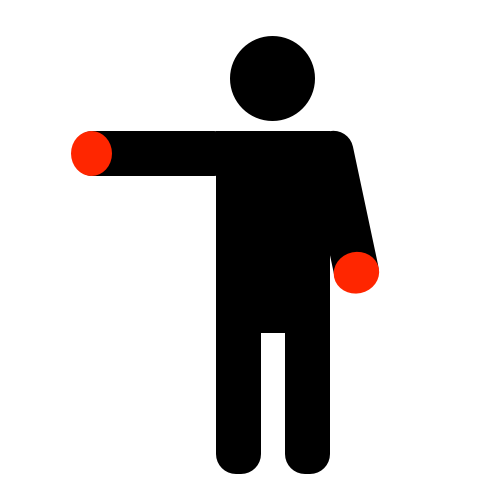
\includegraphics[height=120px]{figs/technical_challenges/kick-in.png}
        \caption{\color{blue}Kick-in \textlangle{}blue\textrangle{} Team}
    \end{subfigure}
    \begin{subfigure}{.33\textwidth}
        \centering
        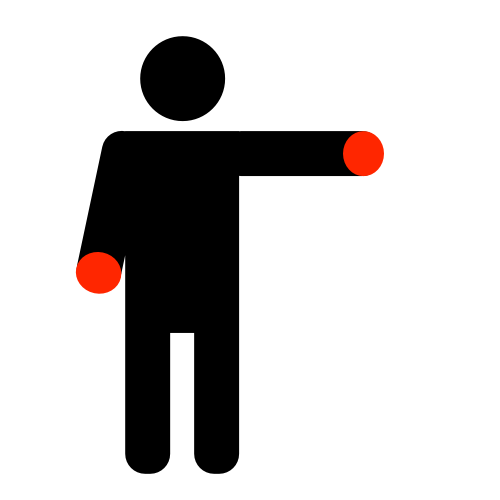
\includegraphics[height=120px]{figs/technical_challenges/kick-in-flipped.png}
        \caption{\color{red}Kick-in \textlangle{}red\textrangle{} Team}
    \end{subfigure}
    \caption{\textbf{Kick-in \textlangle{}color\textrangle{} Team.} One-handed signal. One arm, extended horizontally in the direction of the half of the field corresponding to the team that receives the Kick-in Free Kick. That is, right arm extended for the ``Blue team'', and left arm extended for the ``Red team''. The non-signal hand is flat and motionless by the side of the body.}
\end{figure*}
    
\begin{figure}[ht!]
    \centering
    \begin{subfigure}{.33\textwidth}
        \centering
        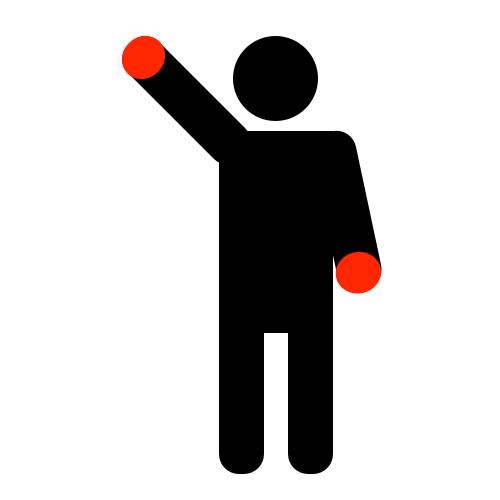
\includegraphics[height=120px]{figs/technical_challenges/goal-kick.png}
        \caption{\color{blue}Goal Kick \textlangle{}blue\textrangle{} Team}
    \end{subfigure}
    \begin{subfigure}{.33\textwidth}
        \centering
        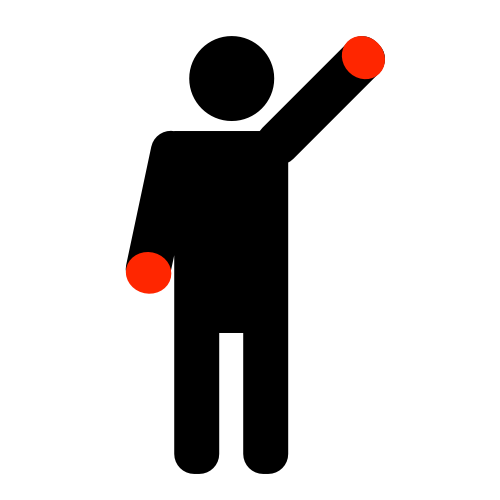
\includegraphics[height=120px]{figs/technical_challenges/goal-kick-flipped.png}
        \caption{\color{red}Goal Kick \textlangle{}red\textrangle{} Team}
    \end{subfigure}
    \caption{\textbf{Goal Kick \textlangle{}color\textrangle{} Team.} One-handed signal. One arm, extended 45-degree \emph{up} in the direction of the end of the field where the goal kick will occur. That is, right arm extended for the ``Blue team'', and left arm extended for the ``Red team''. The non-signal hand is flat and motionless by the side of the body.}
\end{figure}

\begin{figure}[ht!]
    \centering
    \begin{subfigure}{.33\textwidth}
        \centering
        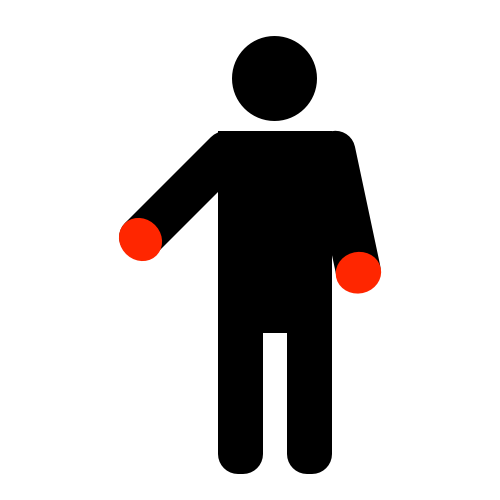
\includegraphics[height=120px]{figs/technical_challenges/corner-kick.png}
        \caption{{\color{blue}Corner Kick \textlangle{}blue\textrangle{} Team}\\ (on the half of the {\color{red} red} team)}
    \end{subfigure}
    \begin{subfigure}{.33\textwidth}
        \centering
        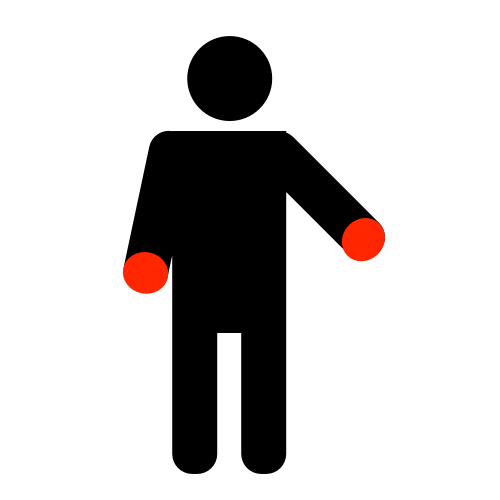
\includegraphics[height=120px]{figs/technical_challenges/corner-kick-flipped.png}
        \caption{{\color{red}Corner Kick \textlangle{}red\textrangle{} Team} (on the half of the {\color{blue} blue} team)}
    \end{subfigure}
    \caption{\textbf{Corner Kick \textlangle{}color\textrangle{} Team.} One-handed signal. One arm, extended 45-degree \emph{down} in the direction of the team executing the corner kick. That is, right arm extended for the ``Blue team'' executing the corner kick on the ``Red team's'' side, and left arm extended for the ``Red team'' executing the corner kick on the ``Blue team's'' side. The non-signal hand is flat and motionless by the side of the body.}
\end{figure}
    
\begin{figure}[ht!]
    \centering
    \begin{subfigure}{.33\textwidth}
        \centering
        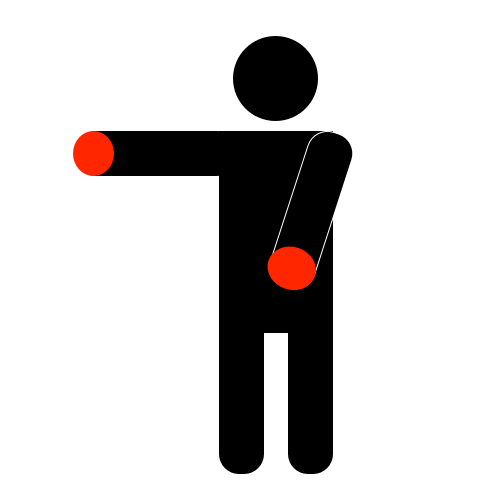
\includegraphics[height=120px]{figs/technical_challenges/goal.png}
        \caption{\color{blue}Goal \textlangle{}blue\textrangle{} Team}
    \end{subfigure}
    \begin{subfigure}{.33\textwidth}
        \centering
        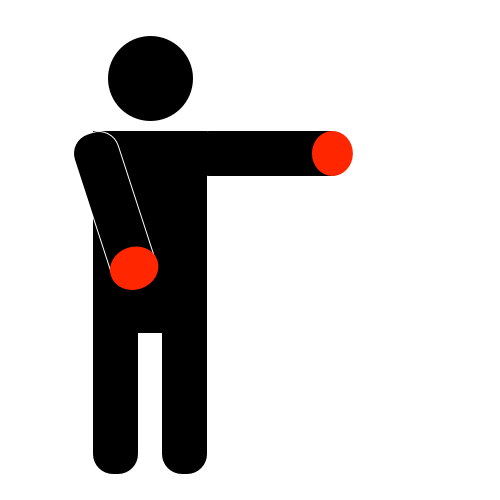
\includegraphics[height=120px]{figs/technical_challenges/goal-flipped.png}
        \caption{\color{red}Goal \textlangle{}red\textrangle{} Team}
    \end{subfigure}
    \caption{\textbf{Goal \textlangle{}color\textrangle{} Team.} Two-handed signal. One arm, extended pointing at the center circle. Other arm, extended horizontally in the direction of the half of the field corresponding to the team that scored the goal. That is, right arm extended for the ``Blue team'', and left arm extended for the ``Red team''.}
\end{figure}

\begin{figure}[ht!]
    \centering
    \begin{subfigure}{.33\textwidth}
        \centering
        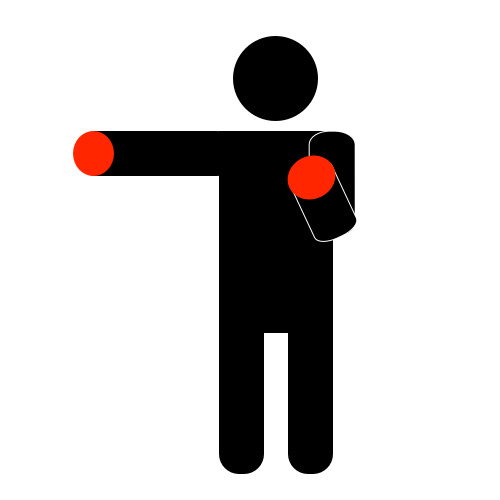
\includegraphics[height=120px]{figs/technical_challenges/pushing.png}
        \caption{{\color{blue}Pushing Free-kick \textlangle{}blue\textrangle{} Team}\\ because a {\color{red}red} robot has pushed.}
    \end{subfigure}
    \begin{subfigure}{.33\textwidth}
        \centering
        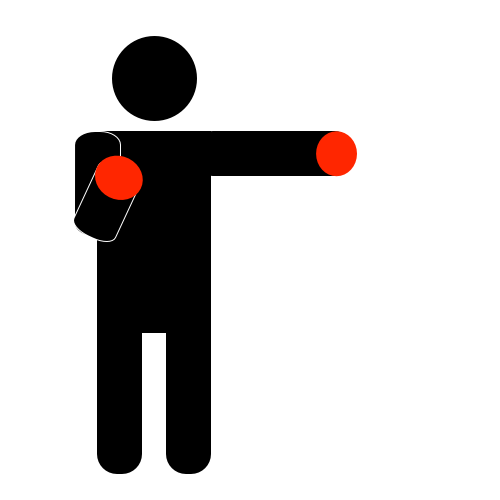
\includegraphics[height=120px]{figs/technical_challenges/pushing-flipped.png}
        \caption{{\color{red}Pushing Free-kick \textlangle{}red\textrangle{} Team}\\ because a {\color{blue}blue} robot has pushed.}
    \end{subfigure}
    \caption{\textbf{Pushing Free-kick \textlangle{}color\textrangle{} Team.} Two-handed signal. One arm, vertical with bent elbow and palm facing in the direction of the extended arm. Other arm, extended horizontally in the direction of the half of the field corresponding to the team that is \emph{executing} the Free-kick. That is, left arm extended for the ``Red team'', and right arm extended for the ``Blue team''.}
\end{figure}

\begin{figure}[ht!]
    \centering
    \begin{subfigure}{.33\textwidth}
        \centering
        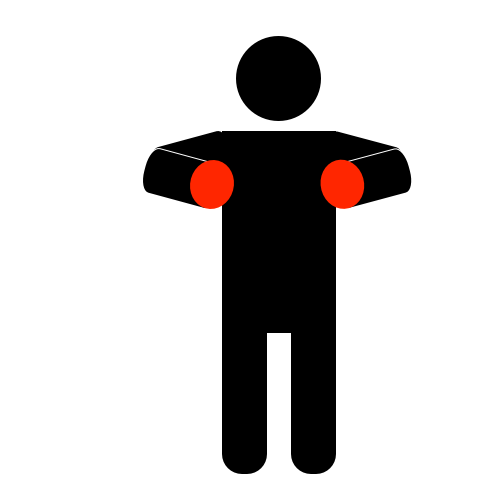
\includegraphics[height=120px]{figs/technical_challenges/full-time-start.png}
        % \caption{Inner start point of the dynamic movement}
    \end{subfigure}
    \begin{subfigure}{.33\textwidth}
        \centering
        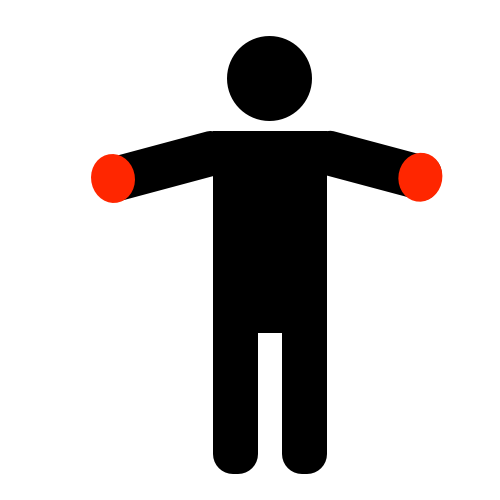
\includegraphics[height=120px]{figs/technical_challenges/full-time-end.png}
        % \caption{Outer start point of the dynamic movement}
    \end{subfigure}
    \caption{\textbf{Full-Time.} Dynamic two-handed signal. Both arms slowly move symmetrically inward and outwards on a horizontal plane, bending at the elbows. Note, for the purpose of this challenge, the whistle associated with this signal should be a \textit{single} blow, unlike in normal SPL games.}
\end{figure}

\clearpage
\subsection{Challenge evaluation}

A team scores 1 point for every hand-signal that is correctly identified. A team scores an additional 1 point for correctly identifying the team corresponding to the signal (where appropriate: For a correct recognized \textit{Full-Time} signal without announcing a team, the team gets also 1 point for the team color). A team looses 1 point for incorrectly identifying a hand-signal (note a team may have a negative final score). The total time for the robot to identify each hand-signal is summed (If a robot fails to identify a hand-signal the time for the hand-signal is \qty{15}{\second}. If a robot incorrectly identifies a hand-signal, the time is how long the robot took to provide the incorrect identification).

TODO: How to handle no goal, many goal, time out. remove best/worst, mean

Teams are ranked by their total points. In the event of tie-breaks, the team with the fastest total time to identify all hand-signals is ranked higher. The team with the highest total points, and lowest total time (for tie-breaks), wins the challenge.

% !TeX root = ../SPL-Challenges.tex
% !TeX spellcheck = en_US
\section{Shared Autonomy Challenge}

This technical challenge will challenge participants to develop a mixed team that consists of one human-operated Nao robot and one fully autonomous Nao. This challenge will consist of matches of two vs two robots on the standard SPL field. The exact number of matches will be subject to the number of available fields and the main competition schedule, however, teams should expect to participate in at least three matches.

\subsection{Challenge Goal}

This challenge takes a step towards the goal of enabling robots to play on the same field as agents with human level intelligence. To level the playing field in terms of physical embodiment, all players will be Nao robots. However, each team will have one of their robots be remotely operated by a human to provide human-level intelligence for robot control. The other robot will be fully autonomous in accordance with the main SPL competition rules.

\subsection{Challenge Rules}

This section details the complete rules to determine play and the winner of each match within the shared autonomy challenge. If not otherwise stated, the Champions Cup rules will be in effect.

\subsubsection{Team Composition}
Each participating team will set up one fully autonomous robot and provide one other robot that is programmed so that it can be operated by a human operator with restricted direct observation of the field, and one team member as the human operator.

\subsubsection{Limitations for Human Operation}
\begin{itemize}
	\item Each participating team will select the operator for their human-operated NAO from their registered team members.
	%
	\item Participating teams will design the appropriate interface for receiving field information from and sending controls to their human-operated robot.
	%
	\item The human operator will sit with their back to the field but close enough to hear referee whistles. The intention is that the operator cannot directly perceive the field but must do so through the controlled robot’s sensors.
	%
	\item The human-operated robot will be penalized if the operator turns and looks at the field.
	%
	\item The human operator may not receive other forms of game perception beyond what the operated robot can stream to it. This limitation includes 1) the human operator watching the challenge live feed on YouTube and 2) other team members with a view of the field communicating game information. However, due to the difficulty of prevention, teams will not be penalized if third-party spectators are overheard remarking on the game and then the human operator bases decisions on those remarks.
	%
	\item Teams are free to determine the operator interface subject to (1) the operator may not look at the field, (2) no teammate is allowed to communicate game information to the operator. The intention is that the operator may only have game information streamed from the human-operated robot and game controller. The referee has the discretion to bar unanticipated modes of communication that go against the spirit of this intention. 
	%
	\item The human-operated robot is not permitted to score goals directly on offense and may not take the goalkeeper role on defense.
\end{itemize}

\subsubsection{Limitations for Autonomy in the Human-Operated Robot}

For the human-operated robot, teams are encouraged to automate parts of control that would be difficult for human control. For example, the human operator may provide walk velocity commands that the robot then implements with a walk engine, or the operator may request a kick, and a kick engine generates the kick on the robot. The human operator may also set higher-level controls, such as the desired location to walk to. However, in the spirit of a mixed human-robot team, the human-operated robot must implement some form of a command from the human operator. That is, it is not permissible to participate in the challenge with two fully autonomous robots or to \textit{only} have the human operator augmenting the robot's perception and localization. 

\subsubsection{Number and duration of attempts}
Each match will give each team one attempt to play offense while the other team defends. An attempt will last 90 seconds or until the attacking team scores. The defending team is not permitted to score goals. If the defending team shoots the ball and it crosses the opponent’s goal line (so that in normal games, a goal would be scored), then a goal kick will be awarded to the attacking team. Effectively, we will treat the entire end line of the attacking team's side of the field as an out-of-bounds line. It is illegal to score directly off of kick off. Matches end in wins, losses, or draws depending on points scored, as described next. 

\subsubsection{Scoring matches}
Points will be awarded during matches on the basis of scoring goals and team coordination. To emphasize scoring on attempts, the attacking team receives two points for each successful goal scored. Teams may also receive additional points for passing where a qualifying pass consists of one robot on a team kicking the ball a distance of more than one (1) meter and then the teammate of the kicking robot making contact with the ball before a robot on the other team kicks or dribbles the ball. Here, a kick (or dribble) is taken to be any contact between a robot's foot while lifted off the ground with the ball. The intention is that incidental contact from the opponent does not disqualify a pass but that intentional contact does. For each qualifying pass, a team receives an additional point. The defending team may also score points via passes. Matches will be decided based on points and not on goals scored.

\subsubsection{Attempt Set-up}
All robots will be manually placed in their \textit{set} location by their team in order to speed up the time between attempts.  Attacking robots will be placed on one side of the field and the defending robots will be on the other side. The attacking team will try to score on the side where the defense starts. For defense, one robot will be designated as the goalkeeper and one as a field player. The goalkeeper must be the autonomous robot. The human-operated field player must be within the penalty area line to start.


\subsubsection{GameController and Penalties}
All robots have to communicate with the GameController. All rules from normal gameplay in the Champions Cup (including penalties) still apply unless explicitly changed here. The game controller operator will communicate the attempt time verbally at 30-second intervals to human operators.

\subsubsection{Network Conditions}
No guarantees are made about the conditions of the wireless network at the competition venue. No limits are placed on communication between the robot and the operator, however, attempts to jam the other team should not be taken. 

\subsubsection{Overall Challenge Scoring}
All participating teams will complete at least three matches and additional matches may be held as the main competition schedule allows. For purposes of deciding an overall challenge winner, the ranking will be based on the following in this order:
\begin{enumerate}
	\item Overall matches won.
	\item Highest score.
	\item Total successful passes.
	\item Goals scored.
\end{enumerate}
If a tie remains after all of these metrics are considered, then the winner will be determined by additional matches between the teams tied for top rank. The TC will determine a method for selecting opponents such that teams are appropriately matched in terms of strength.

\subsubsection{Code Release and Research Dissemination}
To foster the sharing of novel research and enable future development, all participating teams must:
\begin{enumerate}
	\item Prior to the first day of the challenge, submit up to two (2) .pdf slides presenting the team's approach to the competition. At a minimum, the slides should describe 1) the interface for the human operator, 2) the type of command the operator provides to the robot, and 3) the strategy for coordinating the human-operated and autonomous robot. To protect innovation during the competition, these slides will not be shared until after the first day of the challenge.
	\item  Release the code they develop for the human-operated robot (both robot code and interface code).
\end{enumerate}

\subsection{Miscellaneous Notes}

\begin{itemize}
\item Teams are given wide flexibility in interface implementation with the goal of inspiring innovation in how the challenge is addressed. For instance, a team could stream images from the human-operated robot but may face low bandwidth at the venue  (Note, the rules do not specify that any special effort will be made to provide stronger bandwidth for the challenge). Due to bandwidth constraints, teams may prefer to process images on board robot and send high level state info back to operator. However, this forces the operator to work with the robots imprecise state estimation. The choice is left as a research challenge for teams. 
\item Similarly, no specification is given on what control interface can be presented to the human operator. Teams may choose to directly command walk directions and kicks or to use a mixed autonomy mode where the operator gives high level directives that the human-operated robot implements. The only limitation is that the input from the operator must be some sort of command, i.e., it is not sufficient to only augment the robot's perception or localization.
\item Finally, the hardware of the interface (e.g., keyboard, joystick, virtual reality headset) is left up to the discretion of teams.
\item The defending team is not permitted to score because doing so may be too easy to counterattack with long kicks due to the field size and the limited size of teams.
\item Total expected time per match: 5 minutes (3 minutes playing and 2 minutes set up). 
\end{itemize}



% !TeX root = ../SPL-Challenges.tex
% !TeX spellcheck = en_US
\section{Data Minimization Challenge} % TODO: I hope there is a better name for this challenge


\end{document}
